\section{Cutting a Mesh}
\label{sec:Cutting-a-Mesh}

\subsection{Computing a Cutting Path}

All surface parameterization methods proposed in this package only
deal with topological discs (from a mathematical point of view).

Fortunately, the meshes supported by the package can be of any genus and
have any number of connected components. If it is not a topological
disc, the input mesh has to come with a description of a cutting path (an oriented list of
vertices) which is the border of a topological disc.  If no cutting path is
given as input, we assume that the surface border is the longest border already
in the input mesh (the other borders will be considered as holes). \\
Note: the package will only parameterize the inside part of the given border,
thus only one connected component.

% pierre: big contradiction here - it can be something else than a
% disk then!

% Insert image cut.png/eps with title "Cutting Path"
\begin{center}
    \label{Surface_mesh_parameterization-fig-cut}
    % Image
    \begin{ccTexOnly}
        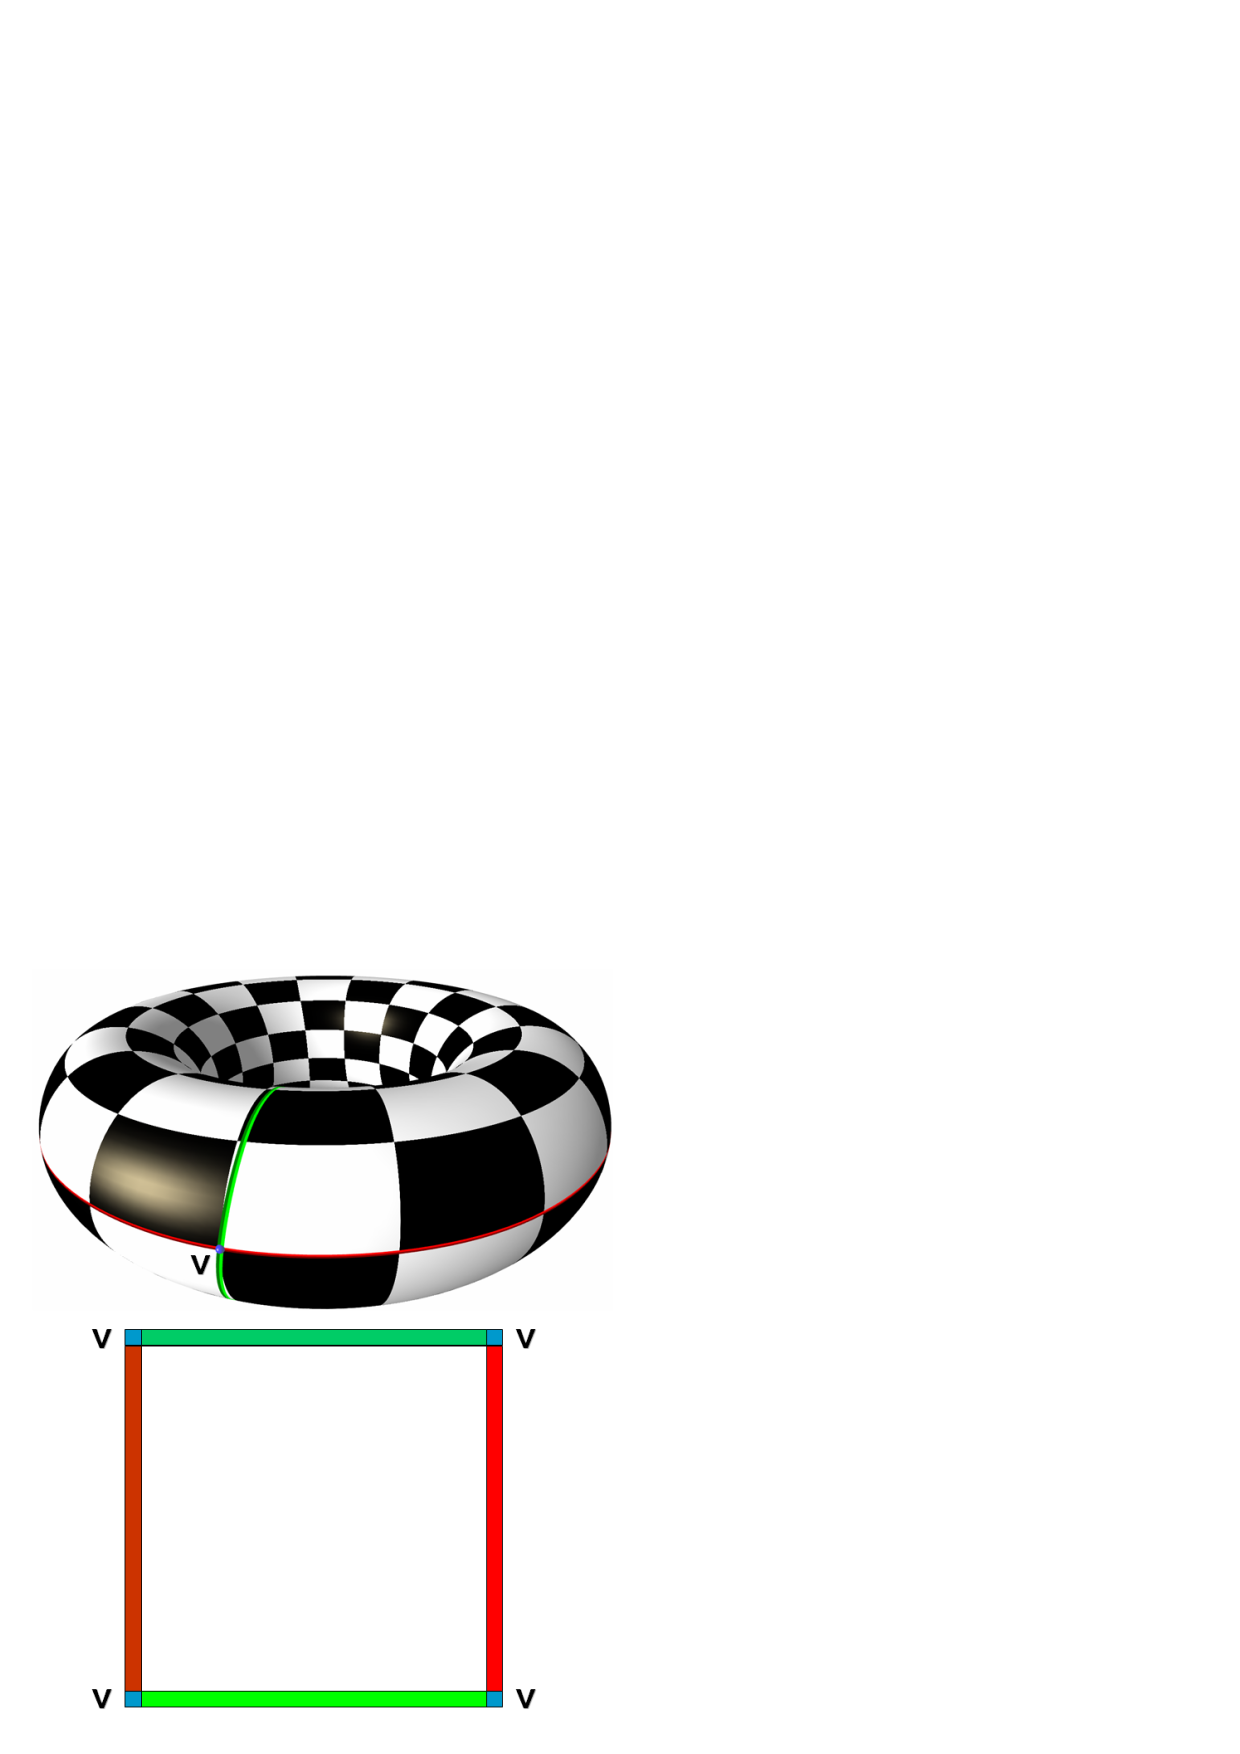
\includegraphics[width=0.4\textwidth]{Surface_mesh_parameterization/cut} % omit .eps suffix
    \end{ccTexOnly}
    \begin{ccHtmlOnly}
        <img width="40%" border=0 src="./cut.png"><P>
    \end{ccHtmlOnly}
    % Title
    \begin{figure}[h]
        \caption{Cutting Path}
    \end{figure}
\end{center}

This package does not provide any algorithm to transform a closed mesh
of arbitrary genus into a topological disk, the user being responsible
for computing such a cutting path. Nevertheless, we provide in
\ccc{polyhedron_ex_parameterization.C} a simple cutting algorithm for
the sake of completeness.


\subsection{Applying a Cut}

The surface parameterization classes in this package only support
\emph{directly} surfaces that are homeomorphic to a disk (models of
\ccc{ParameterizationMesh_3}). This software design simplifies the
implementation of all new parameterization methods.

The \ccc{CGAL::Parameterization_mesh_patch_3<ParameterizationPatchableMesh_3>}
class is responsible for \emph{virtually} cutting
a patch in a \ccc{ParameterizationPatchableMesh_3} mesh.
The resulting patch is a topological
disk (if the input cutting path is correct)
and provides a \ccc{ParameterizationMesh_3} interface. It can be used as
parameter of \ccc{CGAL::parameterize()}.

\ccc{ParameterizationPatchableMesh_3} inherits from concept \ccc{ParameterizationMesh_3},
thus is a concept for a 3D surface mesh.
\ccc{ParameterizationPatchableMesh_3} adds the ability to support patches and
virtual seams. \emph{Patches} are a subset of a 3D mesh.
\emph{Virtual seams} are the ability
to behave exactly as if the surface was cut along a certain path.

The \ccc{ParameterizationMesh_3} interface with the Polyhedron is both a model of
\ccc{ParameterizationMesh_3} and \ccc{ParameterizationPatchableMesh_3}: \\
\ccc{CGAL::Parameterization_polyhedron_adaptor_3<Polyhedron_3_>}

Note that this class is a decorator which adds {\em on the fly}
the necessary fields to unmodified \cgal\ data structures (using STL
maps). For better performances, it is recommended to use \cgal\ data
structures enriched with the proper fields. See \ccc{Polyhedron_ex}
class in \ccc{polyhedron_ex_parameterization.C} example.


\subsection{Cutting a Mesh Example}

\ccc{Mesh_cutting_parameterization.C} \emph{virtually} cuts a
\ccc{CGAL::Polyhedron_3<Traits>} mesh
to make it a topological disk, then applies the default parameterization:

\ccIncludeExampleCode{Surface_mesh_parameterization/Mesh_cutting_parameterization.C}

